\documentclass[12pt,a4paper]{article}
\usepackage{graphicx}
\usepackage{placeins}
\usepackage{indentfirst}
\usepackage{polski}
\usepackage[utf8]{inputenc}
\title{Sprawozdanie z laboratorium PAMSI}
\author{Damian Oleksak}
\date{}
\begin{document}
\maketitle
\newpage

\section*{Wstęp}

Algorytm Simplex jest algorytmem do rozwiązywania zadań programowania liniowego. Został opublikowany przez George'a Dantziga w 1947 roku. Algorytm ten najpierw znajduje pewien wierzchołek wielościanu rozwiązań dopuszczalnych, a następnie w pętli przemieszcza się wzdłuż krawędzi do jednego z sąsiednich wierzchołków tak, aby poprawić wartość funkcji celu. Niestety okazuje się, że jego pesymistyczna złożoność jest wykładnicza. Doskonale zachowuje się on jednak dla ,,rzeczywistych'' danych i jest powszechnie stosowany w praktyce.
\newline

Algorytm zaczyna od dowolnego wierzchołka wielościanu i w każdej kolejnej iteracji próbuje przemieścić się do takiego sąsiedniego wierzchołka, że wartość funkcji celu poprawia się (lub przynajmniej nie pogarsza).\newline

Oto algorytm simplex na przykładzie naszego zadania:
\newline

Musimy znaleźć maksimum funkcji celu f(x):\newline \\
$ 3000 \ast x_{1} + 5000 \ast x_{2} $\newline \\
Z ograniczeniami:\newline \\
$ 3 \ast x_{1} + 2 \ast x_{2} \leq 18 $\newline
$ 2 \ast x_{2} \leq 12 $\newline
$ 1 \ast x_{1} \leq 4 $\newline


\begin{table}[h]
\caption{Przedstawienie problemu firmy produkującej okna i drzwi}
\label{tab.}
\centering
\begin{tabular}{|c|c|c|}
  \hline 
  Czas produkcji drzwi [h] & Czas produkcji okna [h] & Dopuszczalny czas produkcji [h]\\
  \hline
  1 & 0 & 4 \\
  \hline
  0 & 2 & 12 \\
  \hline
    3 & 2 & 18 \\
  \hline
\end{tabular} 
\end{table}

Przy czym:\\ -zysk z produkcji drzwi wynosi 3000 zł;\\  
-zysk z produkcji okna 5000 zł.\\ \newpage

\section*{Rozwiązanie}

Oto rezultat działania programu:\\
\begin{figure}[h]
\centering
\caption[Listing programu]{}
\label{fig:print}
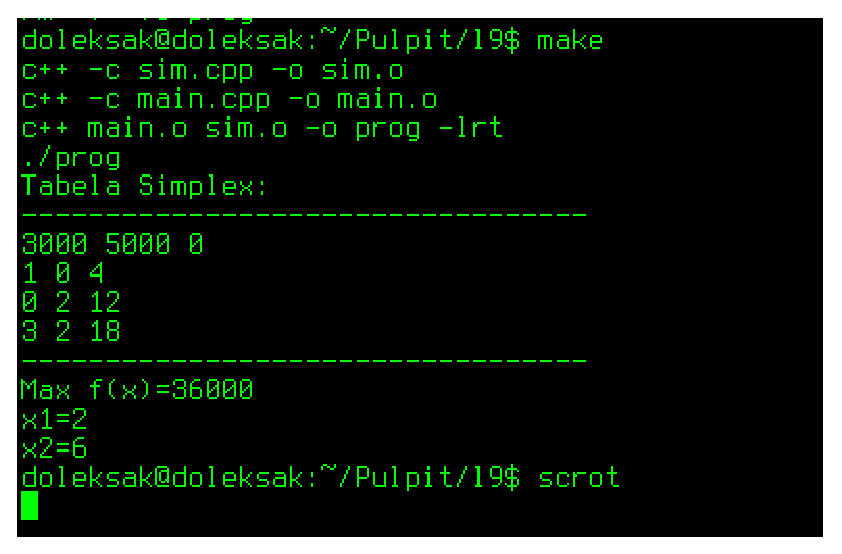
\includegraphics[width=0.7\linewidth]{../l9/print}
\end{figure}

Wygląda na to, że firma osiągnie maksymalny zysk 36000 zł, gdy wyprodukuje dwie pary drzwi i sześć okien.\\

\section*{Uwagi i wnioski}

Dane do programu wprowadza się w wygodny sposób poprzez zmianę zawartości pliku input.txt. Najpierw określamy liczbę zmiennych decyzyjnych i ograniczeń, następnie je wpisujemy w postaci wektorów. W naszym przypadku plik wygląda w następująco:\\
\\
\indent 2 3\\

3000 5000 0\\

1 0 4\\

0 2 12\\

3 2 18

\end{document} 
